\documentclass[a4paper,11pt,twoside]{report}
% THIS FILE SHOULD BE COMPILED BY pdfLaTeX

% ----------------------   PREAMBLE PART ------------------------------

% ------------------------ ENCODING & LANGUAGES ----------------------

\usepackage[utf8]{inputenc}
%\usepackage[MeX]{polski} % Not needed unless You have a name with polish symbols or sth
\usepackage[T1]{fontenc}
\usepackage[english, polish]{babel}
\usepackage{longtable}
\usepackage{ltablex}
\usepackage{amsmath, amsfonts, amsthm, latexsym} % MOSTLY MATHEMATICAL SYMBOLS

\usepackage[final]{pdfpages} % INPUTING TITLE PDF PAGE - GENERATE IT FIRST!
%\usepackage[backend=bibtex, style=verbose-trad2]{biblatex}

% ---------------- MARGINS, INDENTATION, LINESPREAD ------------------

\usepackage[inner=20mm, outer=20mm, bindingoffset=10mm, top=25mm, bottom=25mm]{geometry} % MARGINS


\linespread{1.5}
\allowdisplaybreaks         % ALLOWS BREAKING PAGE IN MATH MODE

\usepackage{indentfirst}    % IT MAKES THE FIRST PARAGRAPH INDENTED; NOT NEEDED
\setlength{\parindent}{5mm} % WIDTH OF AN INDENTATION


%---------------- RUNNING HEAD - CHAPTER NAMES, PAGE NUMBERS ETC. -------------------

\usepackage{fancyhdr}
\pagestyle{fancy}
\fancyhf{}
% PAGINATION: LEFT ALIGNMENT ON EVEN PAGES, RIGHT ALIGNMENT ON ODD PAGES 
\fancyfoot[LE,RO]{\thepage} 
% RIGHT HEADER: zawartość \rightmark do lewego, wewnętrznego (marginesu) 
\fancyhead[LO]{\sc \nouppercase{\rightmark}}
% lewa pagina: zawartość \leftmark do prawego, wewnętrznego (marginesu) 
\fancyhead[RE]{\sc \leftmark}

\renewcommand{\chaptermark}[1]{\markboth{\thechapter.\ #1}{}}

% HEAD RULE - IT'S A LINE WHICH SEPARATES HEADER AND FOOTER FROM CONTENT
\renewcommand{\headrulewidth}{0 pt} % 0 MEANS NO RULE, 0.5 MEANS FINE RULE, THE BIGGER VALUE THE THICKER RULE


\fancypagestyle{plain}{
  \fancyhf{}
  \fancyfoot[LE,RO]{\thepage}
  
  \renewcommand{\headrulewidth}{0pt}
  \renewcommand{\footrulewidth}{0.0pt}
}



% --------------------------- CHAPTER HEADERS ---------------------

\usepackage{titlesec}
\titleformat{\chapter}
  {\normalfont\Large \bfseries}
  {\thechapter.}{1ex}{\Large}

\titleformat{\section}
  {\normalfont\large\bfseries}
  {\thesection.}{1ex}{}
\titlespacing{\section}{0pt}{30pt}{20pt} 

    
\titleformat{\subsection}
  {\normalfont \bfseries}
  {\thesubsection.}{1ex}{}


% ----------------------- TABLE OF CONTENTS SETUP ---------------------------

\def\cleardoublepage{\clearpage\if@twoside
\ifodd\c@page\else\hbox{}\thispagestyle{empty}\newpage
\if@twocolumn\hbox{}\newpage\fi\fi\fi}


% THIS MAKES DOTS IN TOC FOR CHAPTERS
\usepackage{etoolbox}
\makeatletter
\patchcmd{\l@chapter}
  {\hfil}
  {\leaders\hbox{\normalfont$\m@th\mkern \@dotsep mu\hbox{.}\mkern \@dotsep mu$}\hfill}
  {}{}
\makeatother

\usepackage{titletoc}
\makeatletter
\titlecontents{chapter}% <section-type>
  [0pt]% <left>
  {}% <above-code>
  {\bfseries \thecontentslabel.\quad}% <numbered-entry-format>
  {\bfseries}% <numberless-entry-format>
  {\bfseries\leaders\hbox{\normalfont$\m@th\mkern \@dotsep mu\hbox{.}\mkern \@dotsep mu$}\hfill\contentspage}% <filler-page-format>

\titlecontents{section}
  [1em]
  {}
  {\thecontentslabel.\quad}
  {}
  {\leaders\hbox{\normalfont$\m@th\mkern \@dotsep mu\hbox{.}\mkern \@dotsep mu$}\hfill\contentspage}

\titlecontents{subsection}
  [2em]
  {}
  {\thecontentslabel.\quad}
  {}
  {\leaders\hbox{\normalfont$\m@th\mkern \@dotsep mu\hbox{.}\mkern \@dotsep mu$}\hfill\contentspage}
\makeatother



% ---------------------- TABLES AD FIGURES NUMBERING ----------------------

\renewcommand*{\thetable}{\arabic{chapter}.\arabic{table}}
\renewcommand*{\thefigure}{\arabic{chapter}.\arabic{figure}}


% ------------- DEFINING ENVIRONMENTS FOR THEOREMS, DEFINITIONS ETC. ---------------

\makeatletter
\newtheoremstyle{definition}
{3ex}%                           % Space above
{3ex}%                           % Space below
{\upshape}%                      % Body font
{}%                              % Indent amount
{\bfseries}%                     % Theorem head font
{.}%                             % Punctuation after theorem head
{.5em}%                          % Space after theorem head, ' ', or \newline
{\thmname{#1}\thmnumber{ #2}\thmnote{ (#3)}}
\makeatother

\theoremstyle{definition}
\newtheorem{theorem}{Theorem}[chapter]
\newtheorem{lemma}[theorem]{Lemma}
\newtheorem{example}[theorem]{Example}
\newtheorem{proposition}[theorem]{Proposition}
\newtheorem{corollary}[theorem]{Corollary}
\newtheorem{definition}[theorem]{Definition}
\newtheorem{remark}[theorem]{Remark}

% --------------------- END OF PREAMBLE PART (MOSTLY) --------------------------





% -------------------------- USER SETTINGS ---------------------------

\newcommand{\tytul}{System zarządzania zasobami małego laboratorium chemicznego}
\renewcommand{\title}{A System for Resources Management in a Small Chemical Laboratory}
\newcommand{\type}{Engineer} % Master OR Engineer
\newcommand{\supervisor}{dr inż. Agnieszka Jastrzębska} % TITLE AND NAME OF THE SUPERVISOR



\begin{document}
\sloppy
\selectlanguage{english}


\includepdf[pages=-]{titlepage} % THIS INPUTS THE TITLE PAGE


% ------------------ PAGE WITH SIGNATURES --------------------------------

\thispagestyle{empty}\newpage
\null

\vfill

\begin{center}
\begin{tabular}[t]{ccc}
............................................. & \hspace*{100pt} & .............................................\\
supervisor's signature & \hspace*{100pt} & author's signature
\end{tabular}
\end{center}



% ---------------------------- ABSTRACTS -----------------------------

{
\begin{abstract}

\begin{center}
\title
\end{center}

Firstly we will write an abstract of our work in English.\\

\noindent \textbf{Keywords:} keyword1, keyword2, ...
\end{abstract}
}

\null\thispagestyle{empty}\newpage


{\selectlanguage{polish}
\begin{abstract}

\begin{center}
\tytul
\end{center}



\noindent \textbf{Słowa kluczowe:} slowo1, slowo2, ...
\end{abstract}
}


% --------------------------- DECLARATION ------------------------------------


\null\thispagestyle{empty}\newpage

\null \hfill Warsaw, ..................

\par\vspace{5cm}

\begin{center}
Declaration
\end{center}

I hereby declare that the thesis entitled ,,\title '', submitted for the \type ~degree, supervised  by \supervisor , is entirely my original work apart from the recognized reference.
\vspace{2cm}

\begin{flushright}
  \begin{minipage}{50mm}
    \begin{center}
      ..............................................

    \end{center}
  \end{minipage}
\end{flushright}

\thispagestyle{empty}
\newpage

\null\thispagestyle{empty}\newpage
% ------------------- 4. Spis treści ---------------------
% \selectlanguage{english} - for English
\pagenumbering{gobble}
\tableofcontents
\thispagestyle{empty}
\newpage % IF YOU HAVE EVEN QUANTITY OD PAGES OF TOC, THEN REMOVE IT OR ADD \null\newpage FOR DOUBLE BLANK PAGE BEFORE INTRODUCTION


% -------------------- THE BODY OF THE THESIS --------------------------------

\null\thispagestyle{empty}\newpage
\pagestyle{fancy}
\pagenumbering{arabic}
\setcounter{page}{11}


\chapter*{Introduction}
\markboth{}{Introduction}
\addcontentsline{toc}{chapter}{Introduction}


For our engeeniring project, we have designed and implemented a system supporting management of supplies in a small chemical laboratory (chemical reagents, instruments, etc.). The system keeps track of the state of resources in the laboratory, and stores the data in a database. The system has graphical user-friendly interface which facilitates displaying and modifying the gathered data. Multiple functionalities in the system allow the user to: 
\begin{itemize}
\item Classify the resource into groups
\item Assign descriptions with multimedia content to resources
\item	Define and generate reports and notifications displaying current state of resources as well as plot of activity in time, plot of demand for some resource in time, bar chart, pie chart, table with adjustable columns/rows, an alert about low level of some chemical reagent, etc.
\item For each resource, store suppliers’ contact data and order new resources directly from the application
\item Predict future demand for resources based on available historical data
\end{itemize}
The further describiton of the project is contained in the following chapters.



% ----------------------- Work Division ------------------

\chapter{Work Division Plan}

The project was designed so as it could be completed by the group of three people. The tasks were divided equally. That being said, all three participants of the project contributed towards the building of the system, its design and the frame application. What is more, great emphasis has been put on collaboration and team work, resulting in members of the group often performing tasks outside their divised part, which contributed toward the project's final success.

\section{Work Division}

\begin{table}[!h]% Koniecznie label po caption, inaczej jest zła numeracja
\caption[Work Division]{Work Division}
\label{division}
\centering
\begin{tabular}{|p{4cm}|p{12cm}|}
\hline
\texttt{Name} & \texttt{Responsibility} \\ \hline
\texttt{Klaudia Jarosz} & Implementation of the frame application\\ \cline{2-2}
\texttt{} & Creating a database containg data about users, resources, suppliers and user's activity\\  \cline{2-2}
\texttt{} & Design and implementation of a user-friendly interface \\ \cline{2-2}
\texttt{} & Testing \\ \hline
\texttt{Maciej Głowala} & Implementation of the frame application\\ \cline{2-2}
\texttt{} & Handling users with different roles\\  \cline{2-2}
\texttt{} & Saving and restoring system state \\ \cline{2-2}
\texttt{} & Virtual server setup \\ \cline{2-2}
\texttt{} & Testing \\ \hline
\texttt{Aleksandra Bułka} & Implementation of the frame application\\ \cline{2-2}
\texttt{} & Implementation of reports and notifications\\  \cline{2-2}
\texttt{} & Forecasting module\\ \cline{2-2}
\texttt{} & Testing \\ \hline


\end{tabular}
\end{table}


% ----------------------- Business Analysis ------------------


\chapter{Business Analysis}

TODO


\section{Business Analysis}

\section{Other Known Solutions}




% ----------------------- Requirement Specification ------------------

\chapter{Requirement Specification}



\section{Functional Requirements}

The functional reuirements of the applications are different for different users of the application. The tables contained in the following chapters provide descriptions of use cases for different groups of application users.
The three groups of users of the application are:
\begin{enumerate}

\item Administrator (manager of the whole system and its users)
\item Manager (a person with rights for laboratory resources management)
\item Registered user

\end{enumerate}

\subsection{Administrator}


\begin{longtable}{|p{3cm}|p{3cm}|p{10cm}|}
\caption[Functional Requirements for Administrator]{Functional Requirements for Administrator}
\label{functional requirements administrator}
\tabularnewline

\hline
\texttt{Actor} & \texttt{Name} & \texttt{Description} \\ \hline
\texttt{Administrator} & Login & Log in to the system\\  \cline{2-3}
\texttt{} & Password Management & Recover his password\\  \cline{3-3}
\texttt{} & & Change his password\\ \cline{2-3}

\texttt{} & User Account Management & Create an account in the system, assign the account to a role (user, manager)\\  \cline{3-3}
\texttt{} & & Modify an account in the system – change either personal data or assignment to a role (user, manager)\\ \cline{3-3}
\texttt{} & & Remove an account from the system\\ \cline{2-3}
\texttt{} & Resource View & Display nicely current availability of resources and their categorization - multiple viewing perspectives, sorting and filtering are available\\ \cline{2-3}
\texttt{} & Resource Management & Define a new type of resource, describe it with description card, add multimedia content to this resource (for example a photograph) and assign the resource with a supplier\\ \cline{3-3}
\texttt{} & & Modify a resource, change description card, multimedia content associated with this resource (for example a photograph) and its assignment to a supplier\\ \cline{3-3}
\texttt{} & & Delete a resource from database\\ \cline{2-3}

\texttt{} & Resource Group Management & Create a group of laboratory resources, define which resources will belong to this group\\ \cline{3-3}
\texttt{} & & Modify a group of laboratory resources, redefine which resources will belong to this group\\ \cline{3-3}
\texttt{} & & Delete a group of laboratory resources\\ \cline{2-3}
\texttt{} & Product View & Display nicely products produced by laboratory and their categorization\\ \cline{2-3}
\texttt{} & Product Management & Define a new type of product, describe it with description card, add multimedia content to this product (for example a photograph)\\ \cline{3-3}
\texttt{} & & Modify a product, change description card, multimedia content associated with this product (for example a photograph)\\ \cline{3-3}
\texttt{} & & Delete a product from database\\ \cline{2-3}
\texttt{} & Product Group Management & Create a group of laboratory product, define which products will belong to this group\\ \cline{3-3}
\texttt{} & & Modify a group of laboratory products, redefine which products will belong to this group\\ \cline{3-3}
\texttt{} & & Delete a group of laboratory products\\ \cline{2-3}

\texttt{} & Report Definition & Define what the report will contain, for example a plot of production in time, plot of demand for some resource in time\\ \cline{3-3}
\texttt{} &  & Define how the data will be presented, for example bar chart, pie chart, table with adjustable columns/rows \\ \cline{3-3}
\texttt{} &  & Generate the desired report \\ \cline{3-3}
\texttt{} &  & Define the recipients and send the report \\ \cline{2-3}
\texttt{} & Prediction Report Definition & Define what the report will contain, this can be either for example production in time or demand for some resource in time\\ \cline{3-3}
\texttt{} &  & Define for which resources, products or groups of resources or products the prediction should be made\\ \cline{3-3}
\texttt{} &  & Generate the desired prediction report \\ \cline{3-3}



\texttt{} &  & Define the recipients and send the prediction report \\ \cline{2-3}
\texttt{} & Notification Definiton & Define whether notifications (an alert about low level of some chemical reagent) will it be sent\\ \cline{3-3}
\texttt{} &  & Define when the notifications will it be sent (set the value which is critical for each reasource)\\ \cline{2-3}
\texttt{} & Order Management & Define how many and which resources are to be ordered\\ \cline{3-3}


\texttt{} & & Send an order\\ \cline{3-3}


\texttt{} & & Turn on automatic ordering of resources or turn it off\\ \cline{2-3}
\texttt{} & System State Management & Save the current state of the system\\ \cline{3-3}
\texttt{} & & Shedule an automatic back-up of a system state\\ \cline{3-3}
\texttt{} & & Restore system state based on an archived backup\\ \hline


\end{longtable}

\subsection{Manager}


\begin{longtable}{|p{3cm}|p{3cm}|p{10cm}|}
\caption[Functional Requirements for Manager]{Functional Requirements for Manager}
\label{functional requirements manager}
\tabularnewline

\hline
\texttt{Actor} & \texttt{Name} & \texttt{Description} \\ \hline
\texttt{Manager} & Login & Log in to the system\\  \cline{2-3}
\texttt{} & Password Management & Recover his password\\  \cline{3-3}
\texttt{} & & Change his password\\ \cline{2-3}

\texttt{} & Resource View & Display nicely current availability of resources and their categorization - multiple viewing perspectives, sorting and filtering are available\\ \cline{2-3}
\texttt{} & Resource Management & Define a new type of resource, describe it with description card, add multimedia content to this resource (for example a photograph) and assign the resource with a supplier\\ \cline{3-3}
\texttt{} & & Modify a resource, change description card, multimedia content associated with this resource (for example a photograph) and its assignment to a supplier\\ \cline{3-3}
\texttt{} & & Delete a resource from database\\ \cline{2-3}

\texttt{} & Resource Group Management & Create a group of laboratory resources, define which resources will belong to this group\\ \cline{3-3}
\texttt{} & & Modify a group of laboratory resources, redefine which resources will belong to this group\\ \cline{3-3}
\texttt{} & & Delete a group of laboratory resources\\ \cline{2-3}
\texttt{} & Product View & Display nicely products produced by laboratory and their categorization\\ \cline{2-3}
\texttt{} & Product Management & Define a new type of product, describe it with description card, add multimedia content to this product (for example a photograph)\\ \cline{3-3}
\texttt{} & & Modify a product, change description card, multimedia content associated with this product (for example a photograph)\\ \cline{3-3}
\texttt{} & & Delete a product from database\\ \cline{2-3}
\texttt{} & Product Group Management & Create a group of laboratory product, define which products will belong to this group\\ \cline{3-3}
\texttt{} & & Modify a group of laboratory products, redefine which products will belong to this group\\ \cline{3-3}
\texttt{} & & Delete a group of laboratory products\\ \cline{2-3}

\texttt{} & Report Definition & Define what the report will contain, for example a plot of production in time, plot of demand for some resource in time\\ \cline{3-3}
\texttt{} &  & Define how the data will be presented, for example bar chart, pie chart, table with adjustable columns/rows \\ \cline{3-3}
\texttt{} &  & Generate the desired report \\ \cline{3-3}
\texttt{} &  & Define the recipients and send the report \\ \cline{2-3}
\texttt{} & Prediction Report Definition & Define what the report will contain, this can be either for example production in time or demand for some resource in time\\ \cline{3-3}
\texttt{} &  & Define for which resources, products or groups of resources or products the prediction should be made\\ \cline{3-3}
\texttt{} &  & Generate the desired prediction report \\ \cline{3-3}

\texttt{} &  & Define the recipients and send the prediction report \\ \cline{2-3}
\texttt{} & Notification Definiton & Define whether notifications (an alert about low level of some chemical reagent) will it be sent\\ \cline{3-3}
\texttt{} &  & Define when the notifications will it be sent (set the value which is critical for each reasource)\\ \cline{2-3}
\texttt{} & Order Management & Define how many and which resources are to be ordered\\ \cline{3-3}
\texttt{} & & Send an order\\ \cline{3-3}
\texttt{} & & Turn on automatic ordering of resources or turn it off\\ \hline

\end{longtable}



\subsection{User}


\begin{longtable}{|p{3cm}|p{3cm}|p{10cm}|}
\caption[Functional Requirements for User]{Functional Requirements for User}
\label{functional requirements user}
\tabularnewline

\hline
\texttt{Actor} & \texttt{Name} & \texttt{Description} \\ \hline
\texttt{User} & Login & Log in to the system\\  \cline{2-3}
\texttt{} & Password Management & Recover his password\\  \cline{3-3}
\texttt{} & & Change his password\\ \cline{2-3}

\texttt{} & Resource View & Display nicely current availability of resources and their categorization - multiple viewing perspectives, sorting and filtering are available\\ \cline{2-3}
\texttt{} & Resource Management & Define a new type of resource, describe it with description card, add multimedia content to this resource (for example a photograph) and assign the resource with a supplier\\ \cline{3-3}
\texttt{} & & Modify a resource, change description card, multimedia content associated with this resource (for example a photograph) and its assignment to a supplier\\ \cline{3-3}
\texttt{} & & Delete a resource from database\\ \cline{2-3}

\texttt{} & Product View & Display nicely products produced by laboratory and their categorization\\ \cline{2-3}
\texttt{} & Product Management & Define a new type of product, describe it with description card, add multimedia content to this product (for example a photograph)\\ \cline{3-3}
\texttt{} & & Modify a product, change description card, multimedia content associated with this product (for example a photograph)\\ \cline{3-3}
\texttt{} & & Delete a product from database\\ \cline{2-3}
\texttt{} & Report Definition & Define what the report will contain, for example a plot of production in time, plot of demand for some resource in time\\ \cline{3-3}
\texttt{} &  & Define how the data will be presented, for example bar chart, pie chart, table with adjustable columns/rows \\ \cline{3-3}
\texttt{} &  & Generate the desired report \\ \cline{3-3}
\texttt{} &  & Define the recipients and send the report \\ \cline{2-3}
\texttt{} & Prediction Report Definition & Define what the report will contain, this can be either for example production in time or demand for some resource in time\\ \cline{3-3}
\texttt{} &  & Define for which resources, products or groups of resources or products the prediction should be made\\ \cline{3-3}
\texttt{} &  & Generate the desired prediction report \\ \cline{3-3}

\texttt{} &  & Define the recipients and send the prediction report \\ \cline{2-3}

\texttt{} & Order Management & Define how many and which resources are to be ordered\\ \cline{3-3}
\texttt{} & & Send an order\\ \hline

\end{longtable}

\section{Non-functional Requirements}

\begin{table}[!h]% Koniecznie label po caption, inaczej jest zła numeracja
\caption[Non-functional Requirements]{Non-functional requirements}
\label{requirements}
\centering
\begin{tabular}{|p{3cm}|p{2cm}|p{11cm}|}
\hline
Area & Number & Details \\ \hline
\texttt{Usability} & 1 & Application must be responsive. It must be working on PC, tablets and phones with resolution at least 720p.\\  \hline
\texttt{Reliability} & 2 & Application must be of type High Availability. It should be available 24h/7d between 08:00 and 23:00. There could be service breaks during the week between 24:00 and 8:00. \\  \cline{2-3}
\texttt{} & 3 & Application must have quick restart in case of app machine failures. \\ \hline
\texttt{Recovery} & 4 & Application must have daily database recovery performed between 24:00 and 08:00. \\ \hline
\texttt{Performance} & 5 & Application should respond no longer than 3 seconds while strain being on level 100 queries per minute. \\ \hline
\texttt{Supportability} & 6 & Documentation should contain instruction for recovery data from database backup.  \\ \cline{2-3}
\texttt{} & 7 & Application should keep backward compatibility between the released versions.. \\ \hline
\texttt{Security} & 8 & Application must have user levels security. It shall not pass a user who has inappropriate privileges. \\ \hline


\end{tabular}
\end{table}


\section{User Stories}

\section{Use Cases}



% ----------------------- Development Model ------------------

\chapter{Development Model and Methodology}


\section{Methodology}

For our project, the development methodology of choice was the Waterfall Development Model. This methodology was highly recommended to us.

\begin{figure}[h!]

\begin{center}

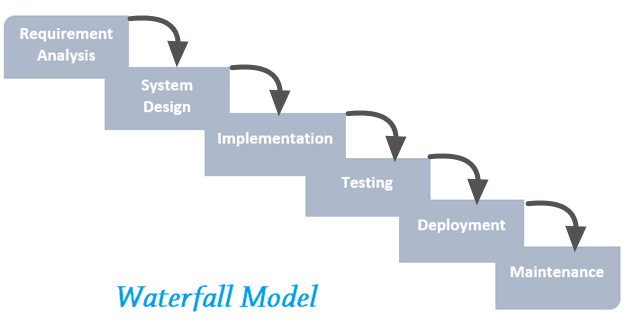
\includegraphics[width=\textwidth]{water}

\end{center}
\caption{Waterfall Model}
\end{figure}


In Waterfall Model phases are executed sequentially, in linear way. We have a steady set of requirements, non changeable in time. The system is developed progressively and the user is involved only in the early phases 
Advantages of this model include it being easy to manage. Disadvantages are that it contains a strict sequence of activities, it has high cost of errors in beginning stages and high importance and cost of documentation and also a contact with the customer is weak. Therefore it can be used when it is possible to precisely define the requirements 

\subsection{Argumentation}

The reasons we have chosen this particular development model are presented below:
\begin{itemize}
\item The sequential order of phases matched perfectly the organized schedule of the development of our Engineering Thesis

\item Fixed set of requirements, as the initial requirements waere submitted by team to the Faculty and could not be changed later
\item Easy management is facilitating our work as we work as a team and have no manager
\item It was highly recommended by the coordinators of the Group Project
\end{itemize}


\section{Development Model}




% ----------------------- Systeem Architecture ------------------


\chapter{System Architecture}



\section{Software Architectural Pattern}


To facilitate the design of classes, we have decided to follow a software architectural pattern. A pattern of choice here was Model–view–controller (MVC) Pattern.
This pattern is used to separate a given application into three interconnected parts. This is done to separate internal representations of information from the ways information is presented to, and accepted from, the user.
\begin{itemize}
\item Model - Model represents an object carrying data. It can also have logic to update controller if its data changes.
\item View - View represents the visualization of the data that model contains.
\item Controller - Controller acts on both model and view. It controls the data flow into model object and updates the view whenever data changes. It keeps view and model separate.
\end{itemize}
\begin{figure}[h!]

\begin{center}

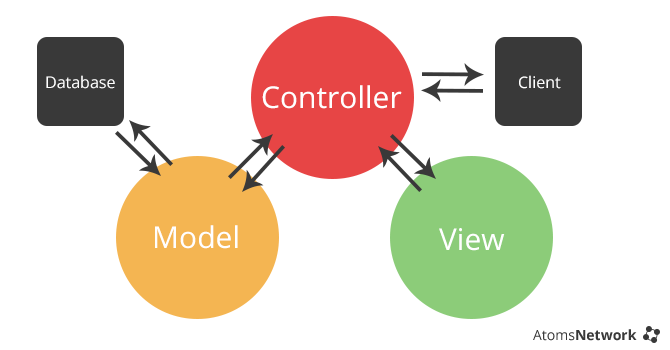
\includegraphics[width=\textwidth]{mvc}

\end{center}
\caption{MVC Pattern}
\end{figure}


As mentioned before, it has helped us develop the division into classes, visible on the class diagram below.
LIME – is the program’s main class.
Then, the Model, View and Controller Classes were designed for each UI element.
The database objects are handled by Servlet (classes taking an article from http POST and passing it to JDBC), DAO (classes responsible for the communication with database) and Query (classes to parse SQL) classes.


\section{Backend Architectural Pattern}

L.I.M.E. project base on many architectural patterns. Precisely chosen patterns make overall architecture strong and well built. 
\subsection{Data Access Object Pattern}

Data access object (DAO) is an object that provides an abstract interface to some type of database or other persistence mechanism. By mapping application calls to the persistence layer, the DAO provides some specific data operations without exposing details of the database. This isolation supports the Single responsibility principle. It separates what data access the application needs, in terms of domain-specific objects and data types (the public interface of the DAO), from how these needs can be satisfied with a specific DBMS, database schema, etc. (the implementation of the DAO).
	The most important fact and advantage is the relatively simple and rigorous separation between two important parts of an application that can but should not know anything of each other, and which can be expected to evolve frequently and independently. Changing business logic can rely on the same DAO interface, while changes to persistence logic do not affect DAO clients as long as the interface remains correctly implemented. All details of storage are hidden from the rest of the application (see information hiding). Thus, possible changes to the persistence mechanism can be implemented by just modifying one DAO implementation while the rest of the application isn't affected.
L.I.M.E. implements one template parent interface with methods which are used by all DAO classes. IBasicCrudRepository extends hibernate CrudRepository and inherits from it all CRUD database operations. Singular DAO classes implement service-specific methods which are defined in DAO interfaces.

% ----------------------- Technical Analysis ------------------


\chapter{Technical Analysis}

More detailed - all the classes and functions


\section{General Program Workflow}


\section{Program Interface}


\section{System Classes}


\section{Database Design}


\section{Prediction Model}



% ----------------------- Experimental Evaluation ------------------

\chapter{Experimental Evaluation}

This is important - these are various tests, trying to cover all the possible thing user can do in the application


\section{Evaluation Plan}



% ----------------------- Acceptance Tests ------------------

\chapter{Acceptance Tests}

This is for other tests


\section{Test Plan}




% ----------------------- Conclusions ------------------
\chapter*{Conclusions}

1 Page of Our Conclusions of Writing This Project
\thispagestyle{empty}




% ------------------------------- BIBLIOGRAPHY ---------------------------
% LEXICOGRAPHICAL ORDER BY AUTHORS' LAST NAMES
% FOR AMBITIOUS ONES - USE BIBTEX


\begin{thebibliography}{20} % IF YOU HAVE MORE REFERENCES, WRITE THE BIGGER NUMBER

\bibitem[1]{Ktos} A. Author, \emph{Title of a book}, Publisher, year, page--page.
\bibitem[2]{Innyktos} J. Bobkowski, S. Dobkowski, Title of an article, \emph{Magazine X, No. 7}, year, PAGE--PAGE.
\bibitem[3]{B} C. Brink, Power structures, \emph{Algebra Universalis 30(2)}, 1993, 177--216.
\bibitem[4]{H} F. Burris, H. P. Sankappanavar, \emph{A Course of Universal Algebra}, Springer-Verlag, New York, 1981.
\end{thebibliography}
\pagenumbering{gobble}
\thispagestyle{empty}



% ----------------------- GLOSSARY ------------------
\chapter*{Glossary}
\begin{tabular}{cl}

\textbf{LIME} & Laboratory Internal Management Entity - the name of the application discussed in this document. LIME is the system for resources management in a small chemical laboratory. \\

\end{tabular}
\\

\thispagestyle{empty}


% ----------------------------  LIST OF FIGURES --------------------------------
\listoffigures
\thispagestyle{empty}
If you don't need it, delete it.


% -----------------------------  LIST OF TABLES --------------------------------
\renewcommand{\listtablename}{List of tables}
\listoftables
\thispagestyle{empty}
If you don't need it, delete it.

% -----------------------------  LIST OF APPENDICES ---------------------------
\chapter*{List of appendices}
\begin{enumerate}
\item Appendix A. User Manual
\item Appendix B. Testing Scenarios
\end{enumerate}
\thispagestyle{empty}


% -----------------------------  APPENDIX A ---------------------------
\chapter*{A. User Manual}

There we will have manual
\thispagestyle{empty}

% -----------------------------  APPENDIX B ---------------------------
\chapter*{B. Testing Scenarios}

Testing Scenarios
\thispagestyle{empty}



\end{document}
